\subsection{Biểu đồ}
\subsubsection{Biểu đồ thời gian chạy}

\paragraph{1. Dữ liệu ngẫu nhiên}
\begin{figure}[H]
    \centering
    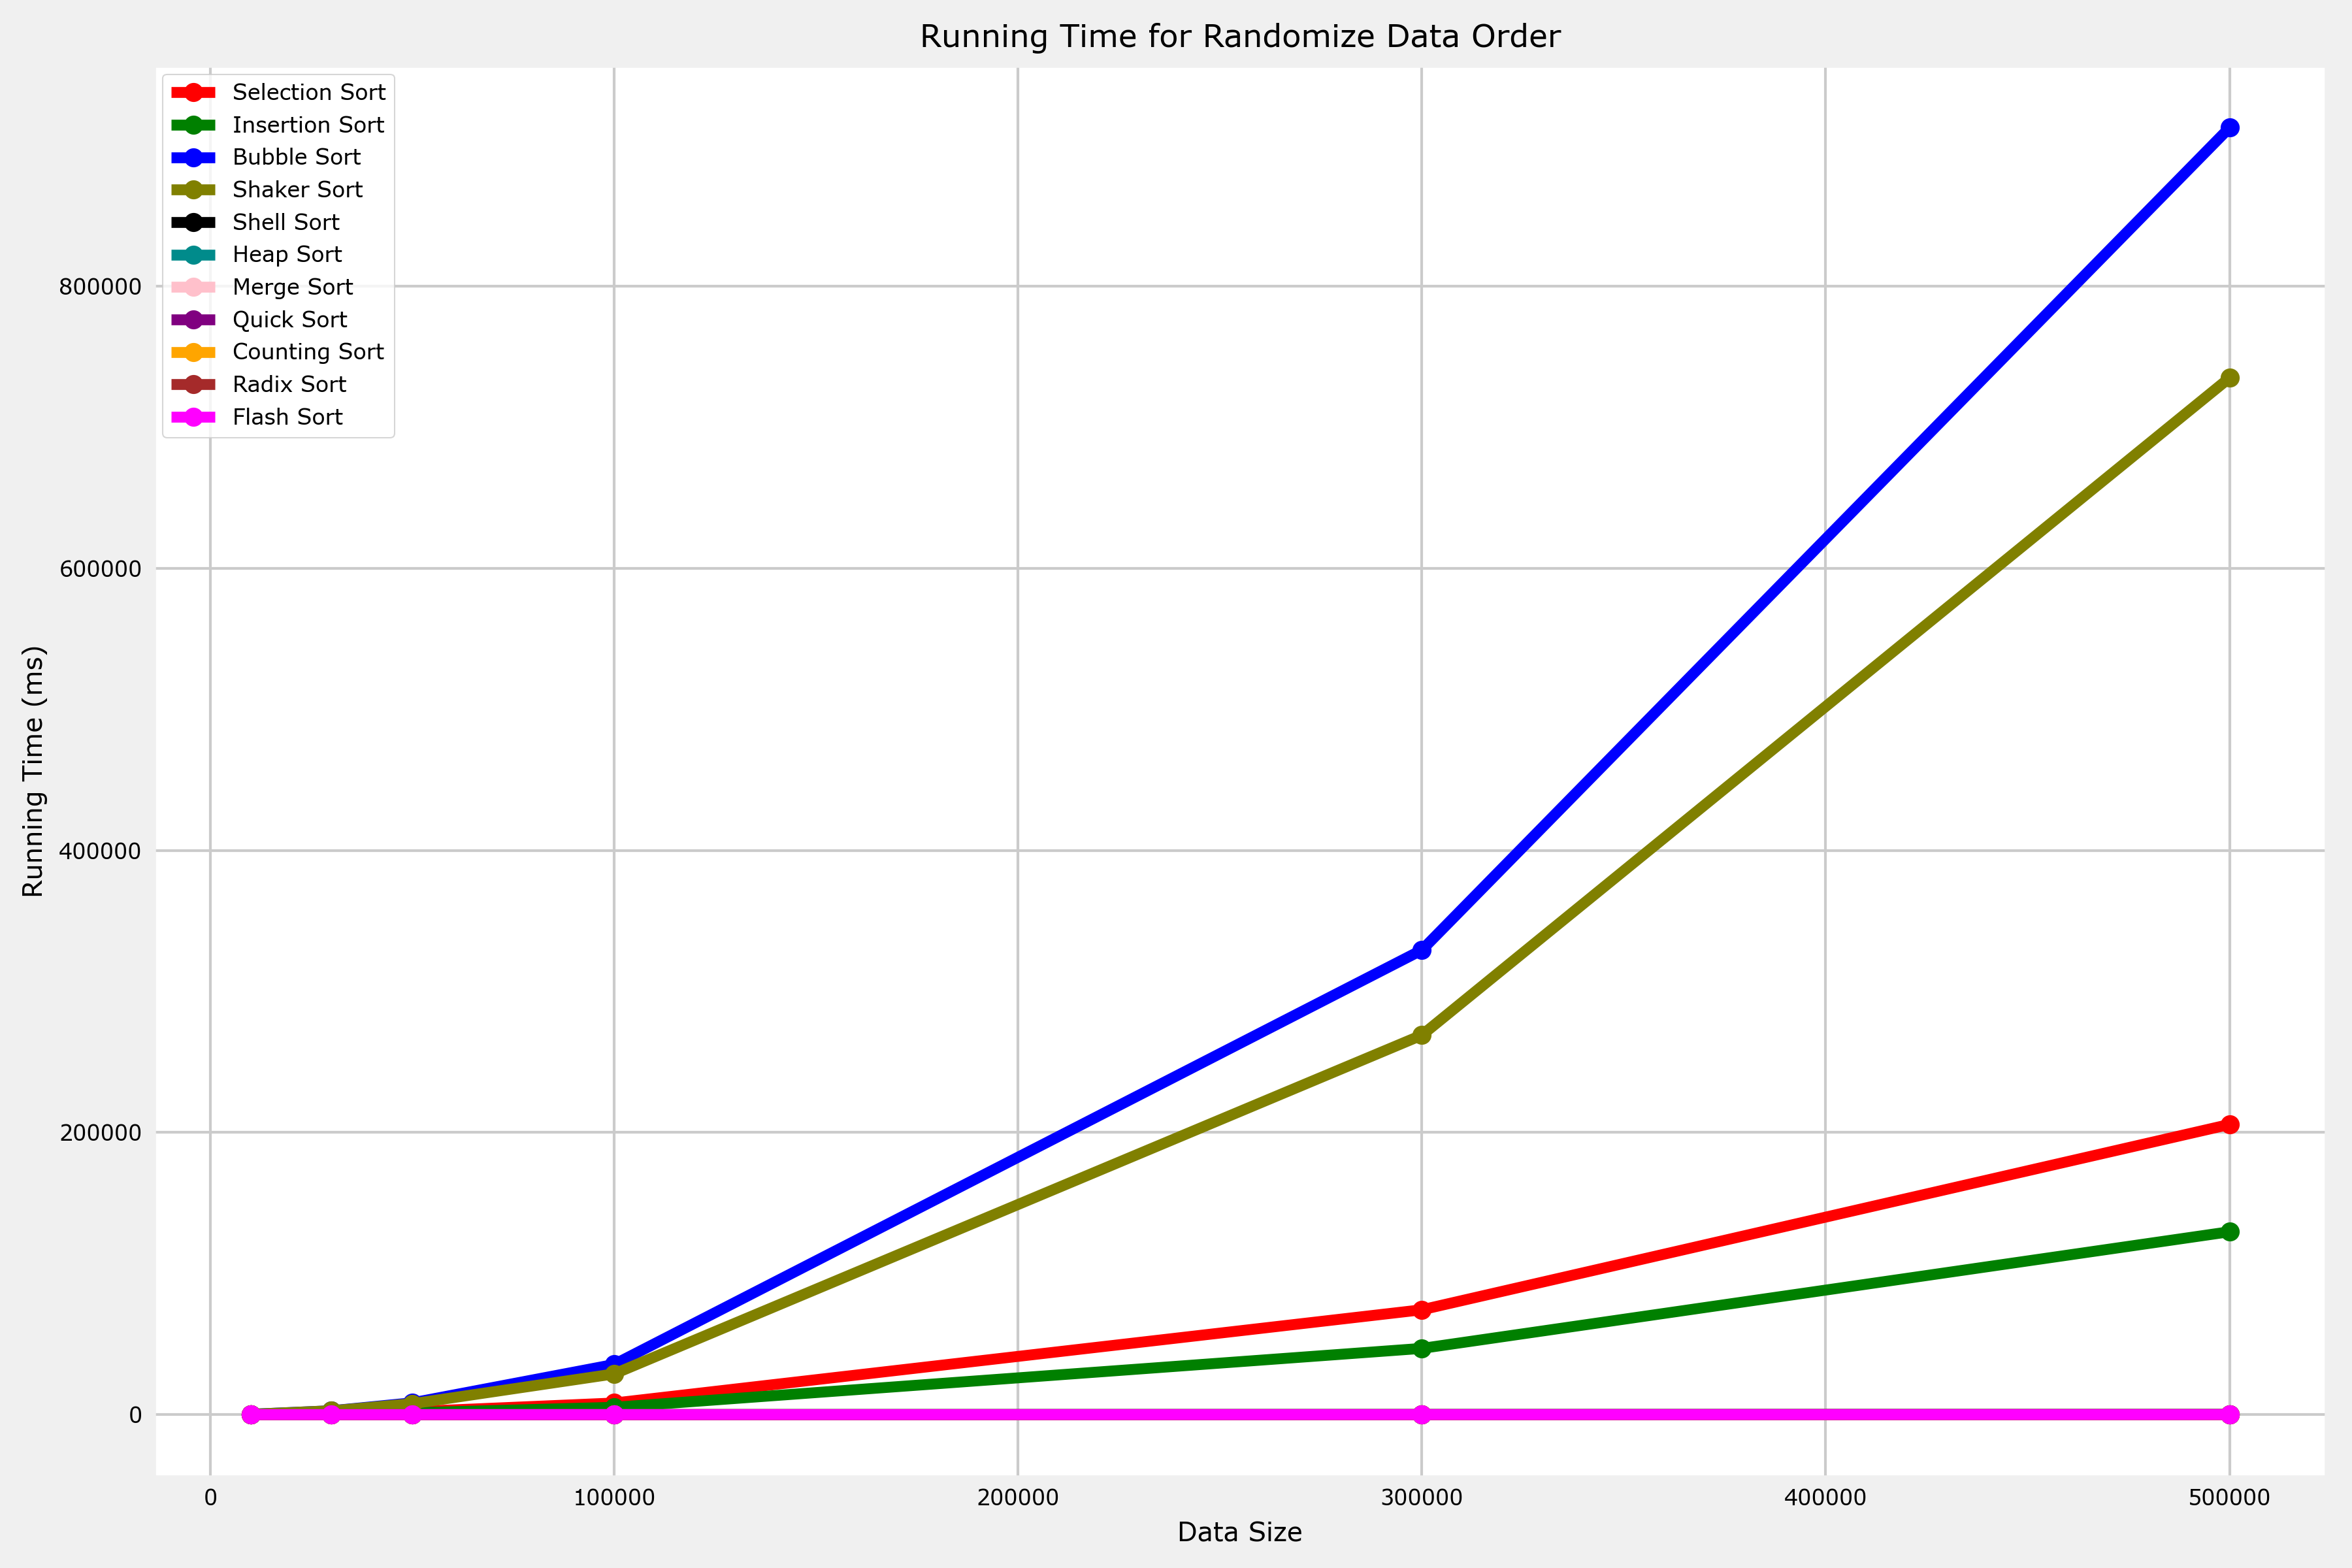
\includegraphics[width=0.8\textwidth]{exprimental_result/images/randomize_running_time.png}
    \caption{Thời gian chạy của 11 thuật toán với dữ liệu ngẫu nhiên}
\end{figure}



\begin{figure}[H]
    \centering
    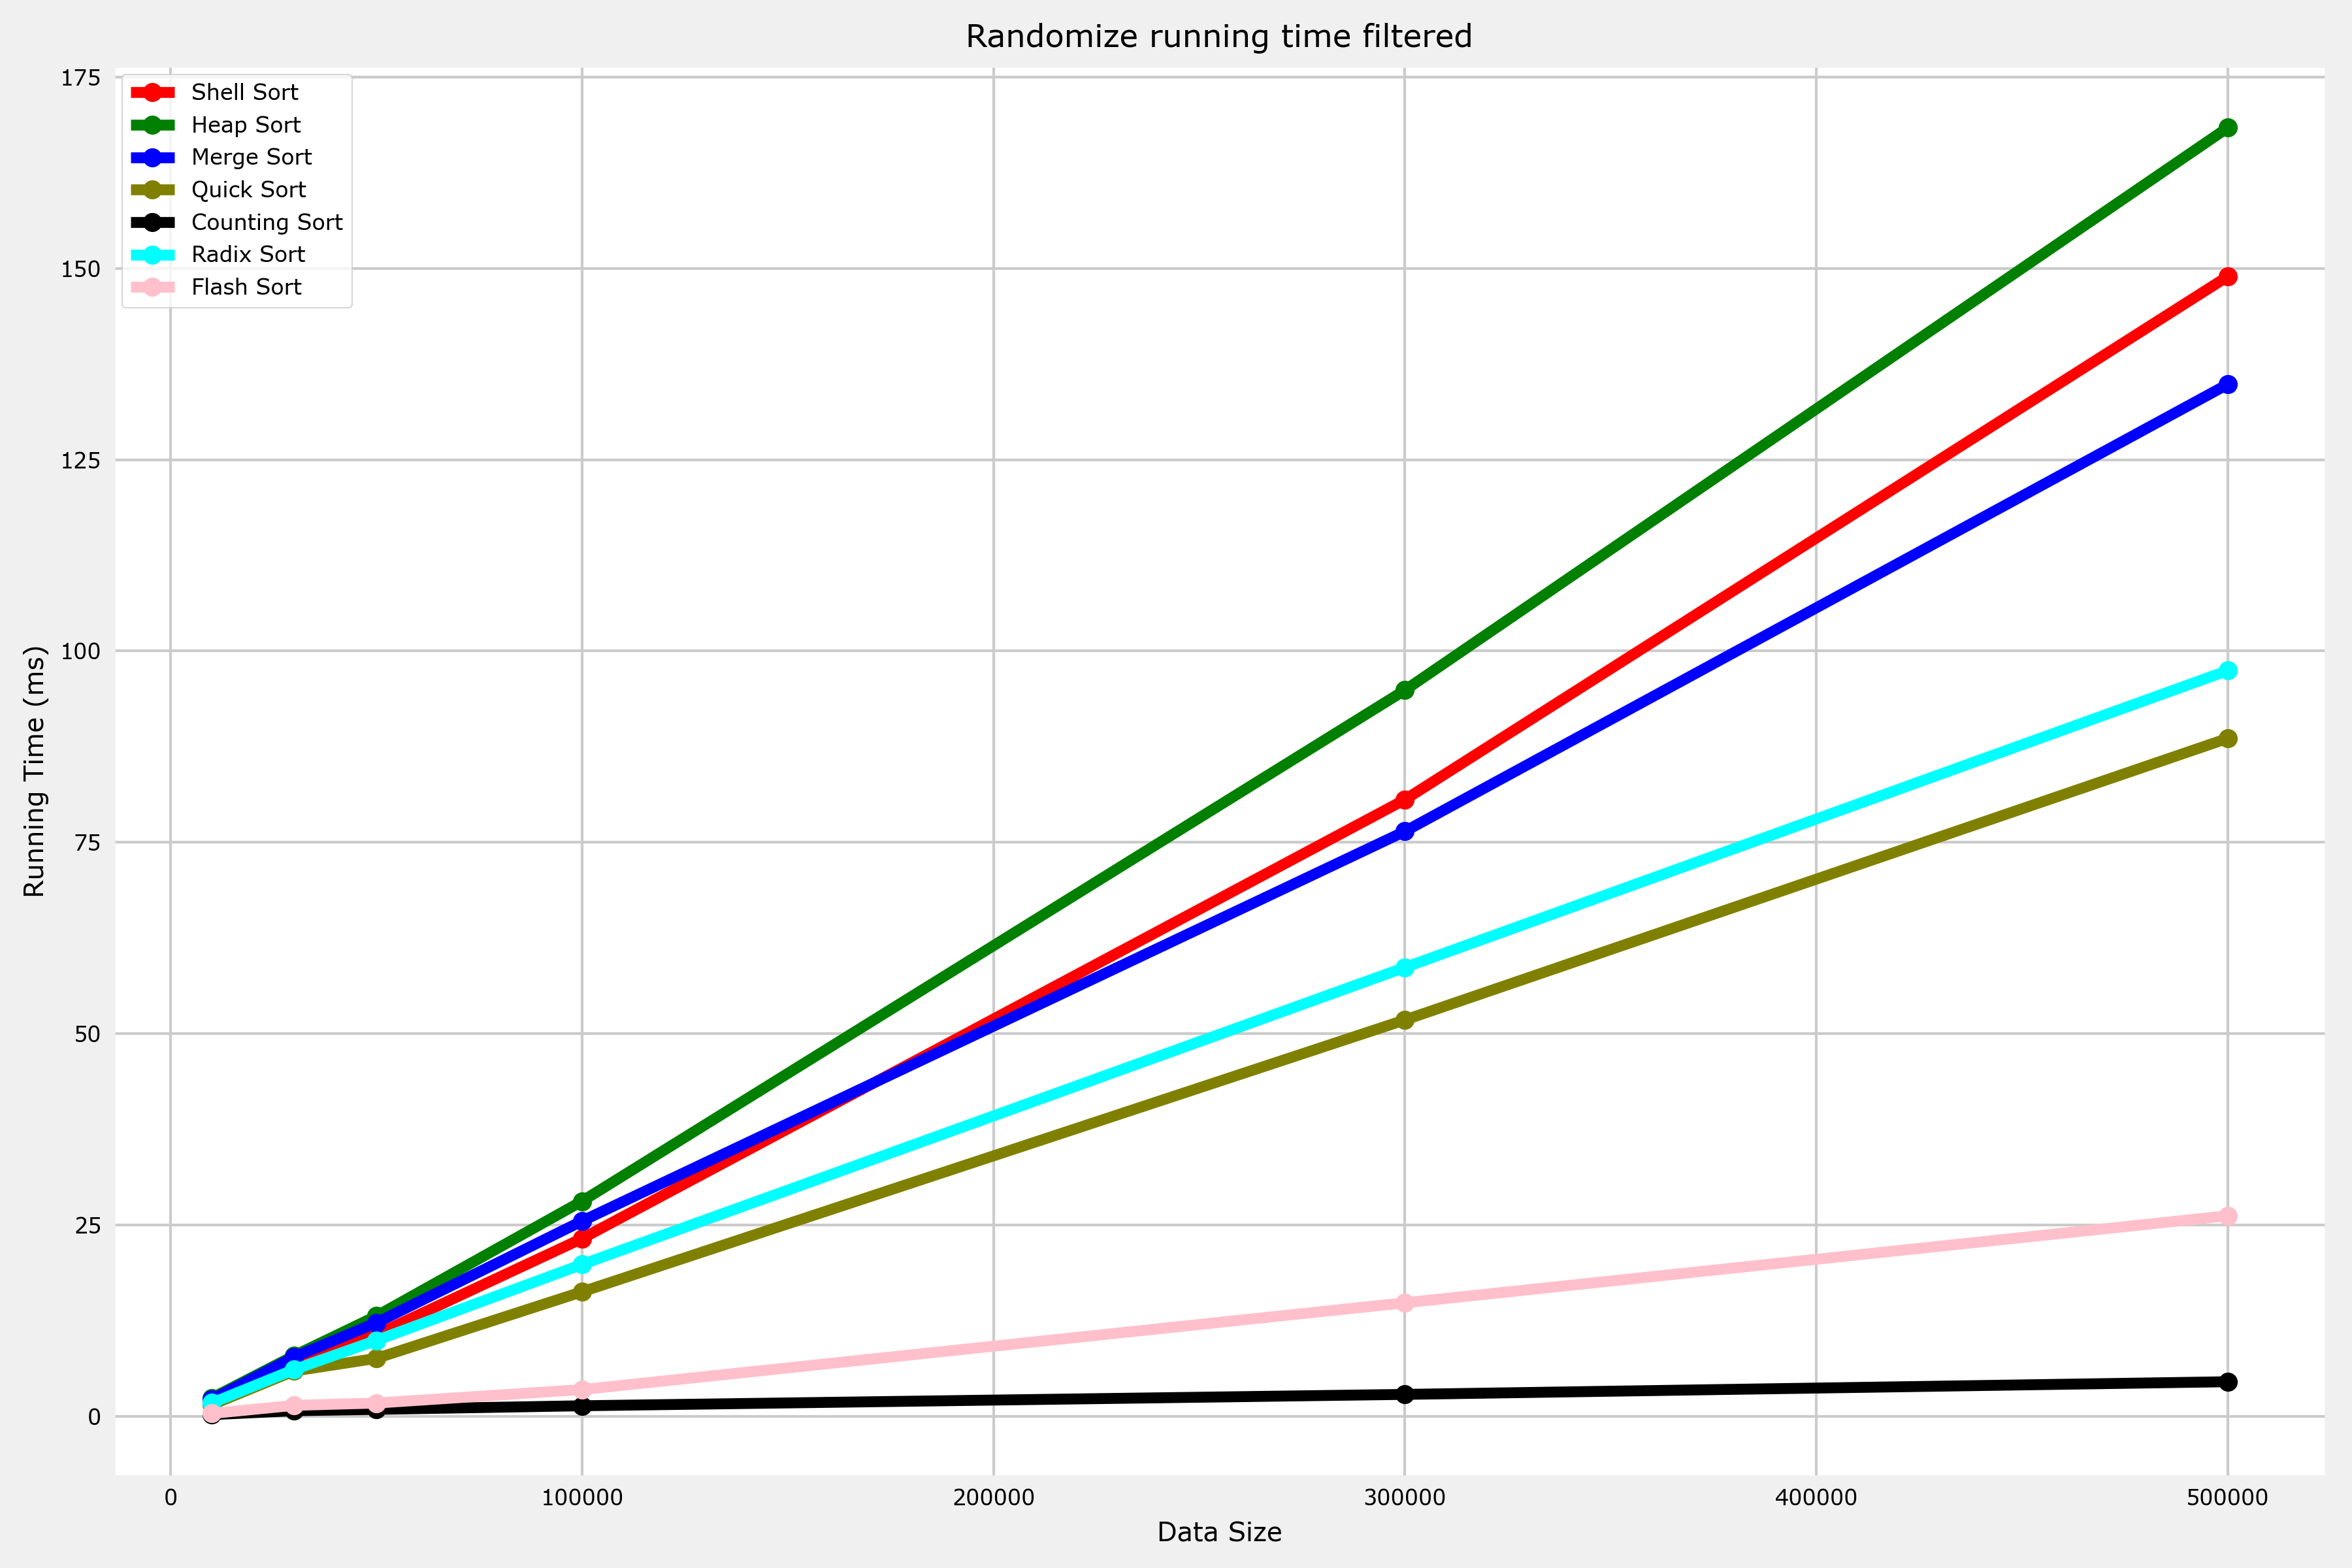
\includegraphics[width=0.8\textwidth]{exprimental_result/images/randomize_running_time_filtered.png}
    \caption{Thời gian chạy của 11 thuật toán với dữ liệu ngẫu nhiên sau khi loại bỏ outlier}
\end{figure}



\paragraph{2. Dữ liệu gần sắp xếp hoàn chỉnh}
\begin{figure}[H]
    \centering
    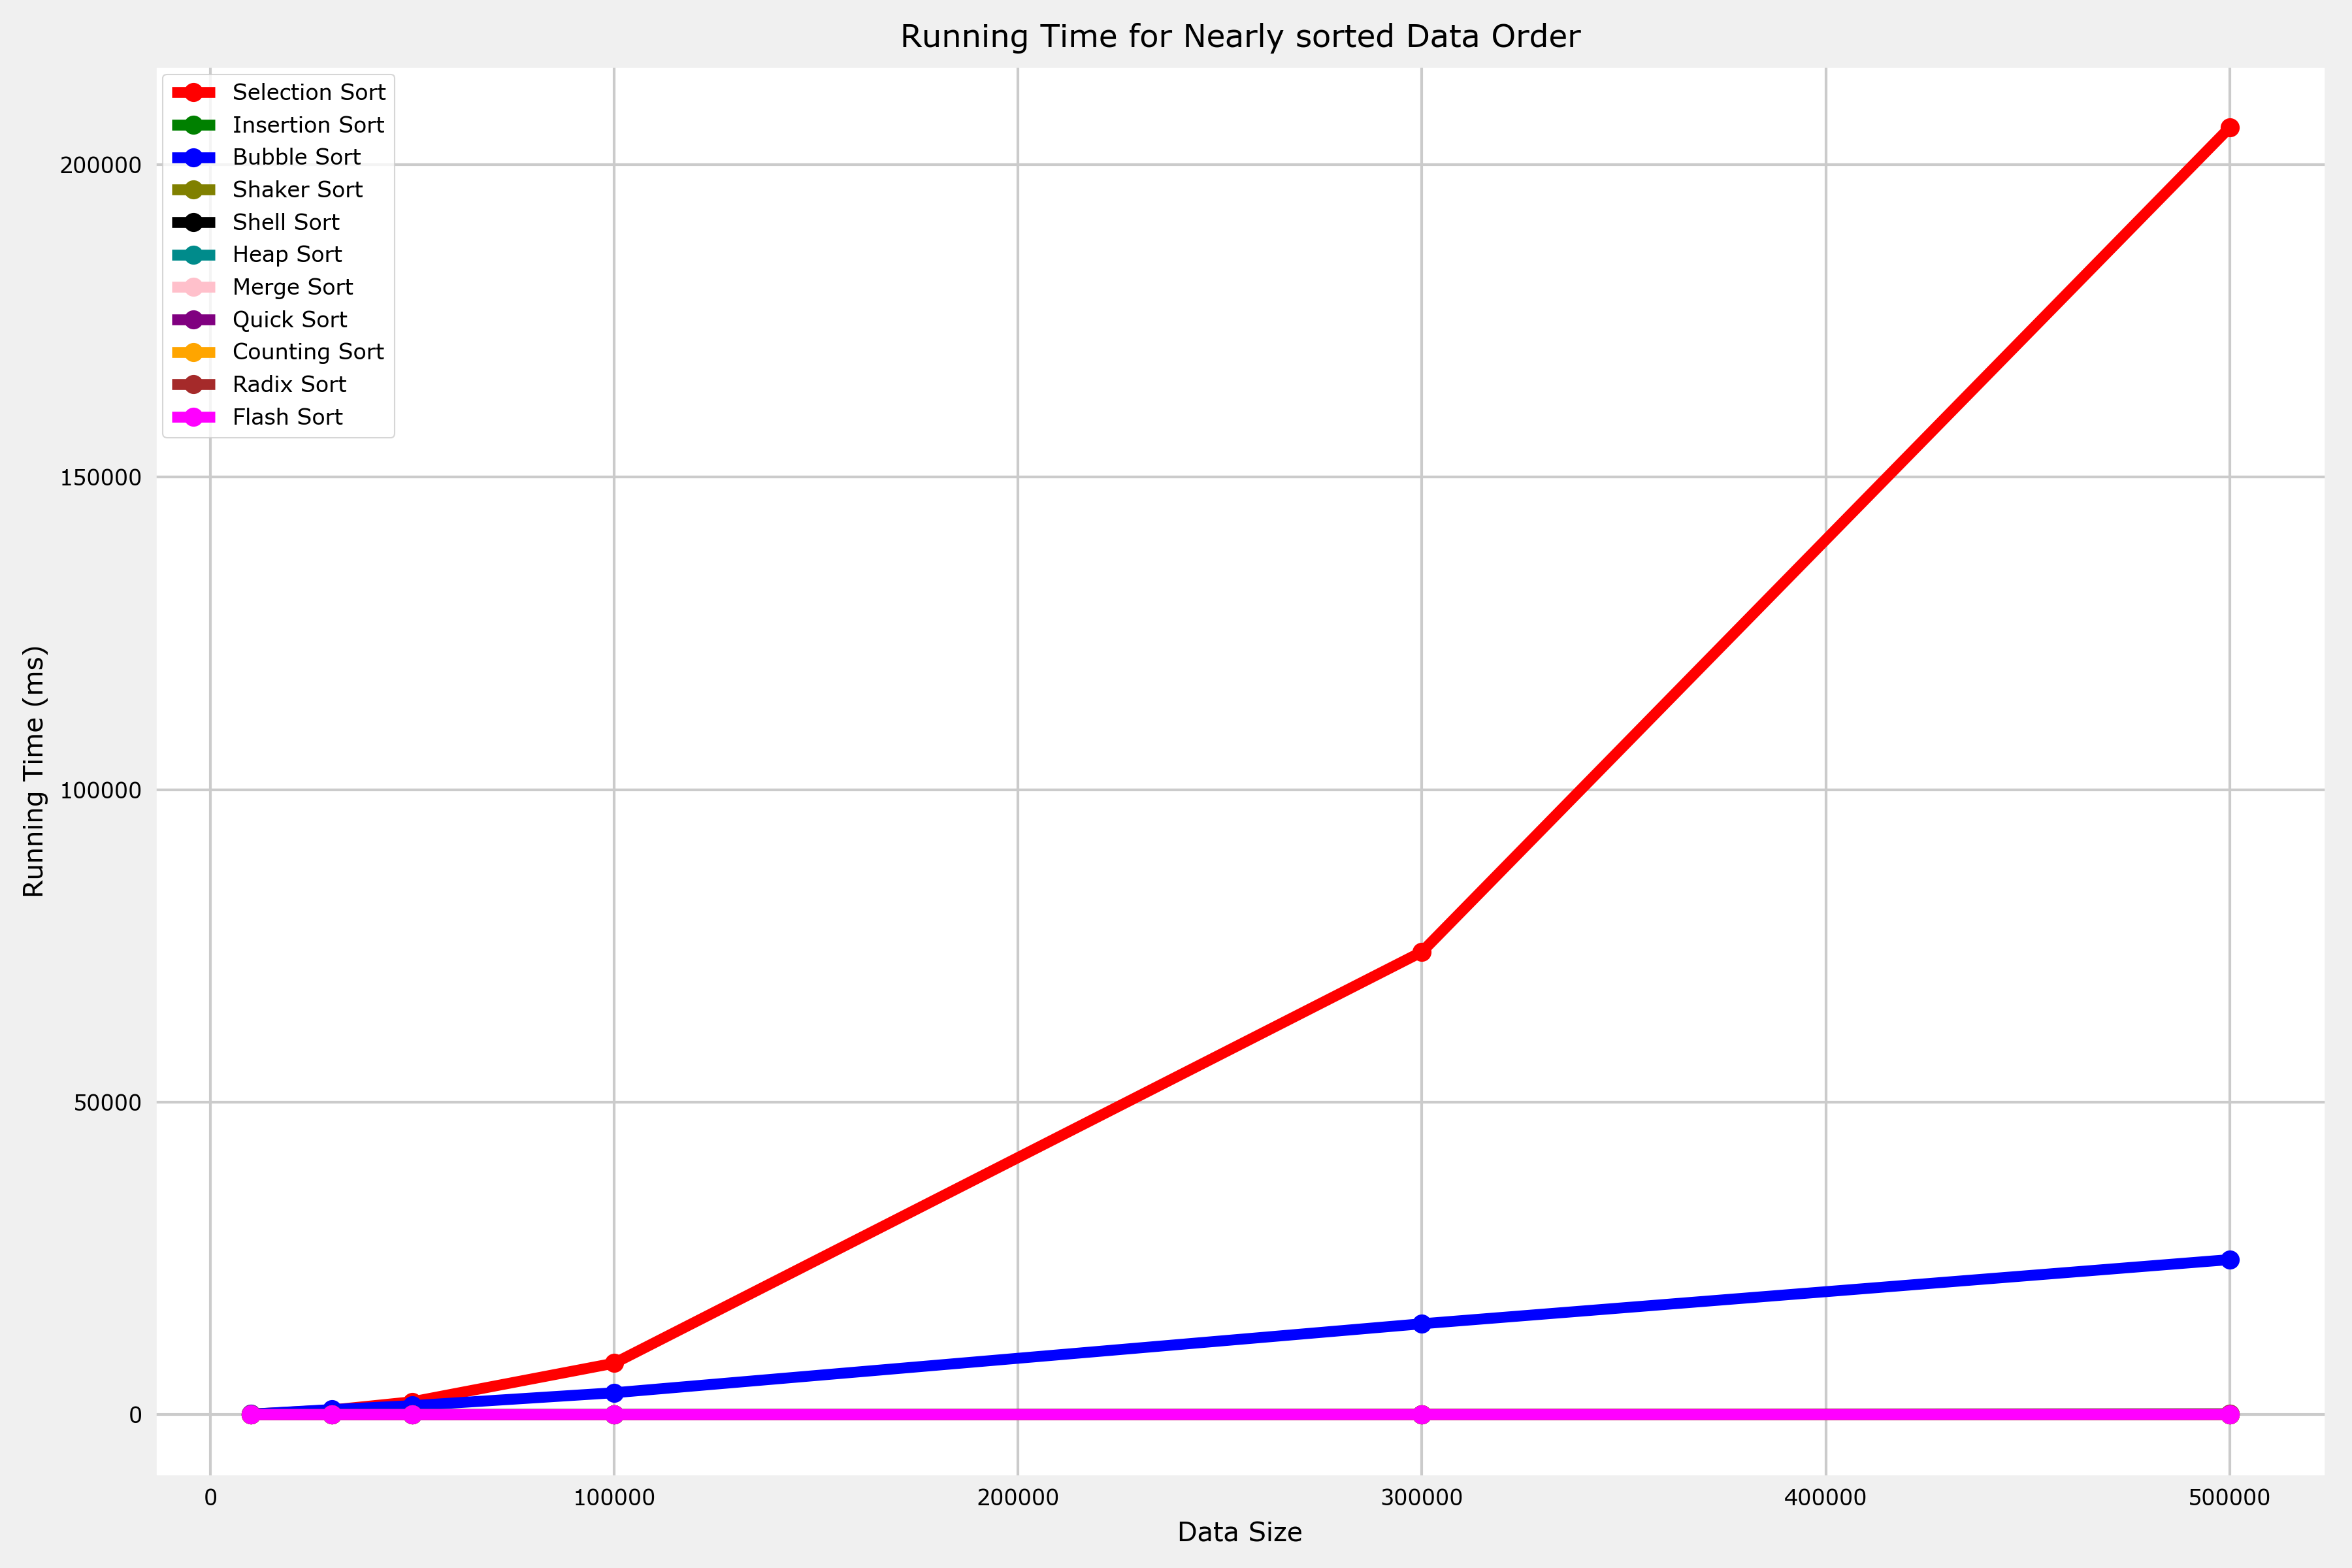
\includegraphics[width=0.8\textwidth]{exprimental_result/images/nearly_sorted_running_time.png}
    \caption{Thời gian chạy của 11 thuật toán với dữ liệu gần sắp xếp hoàn chỉnh}
\end{figure}

\begin{figure}[H]
    \centering
    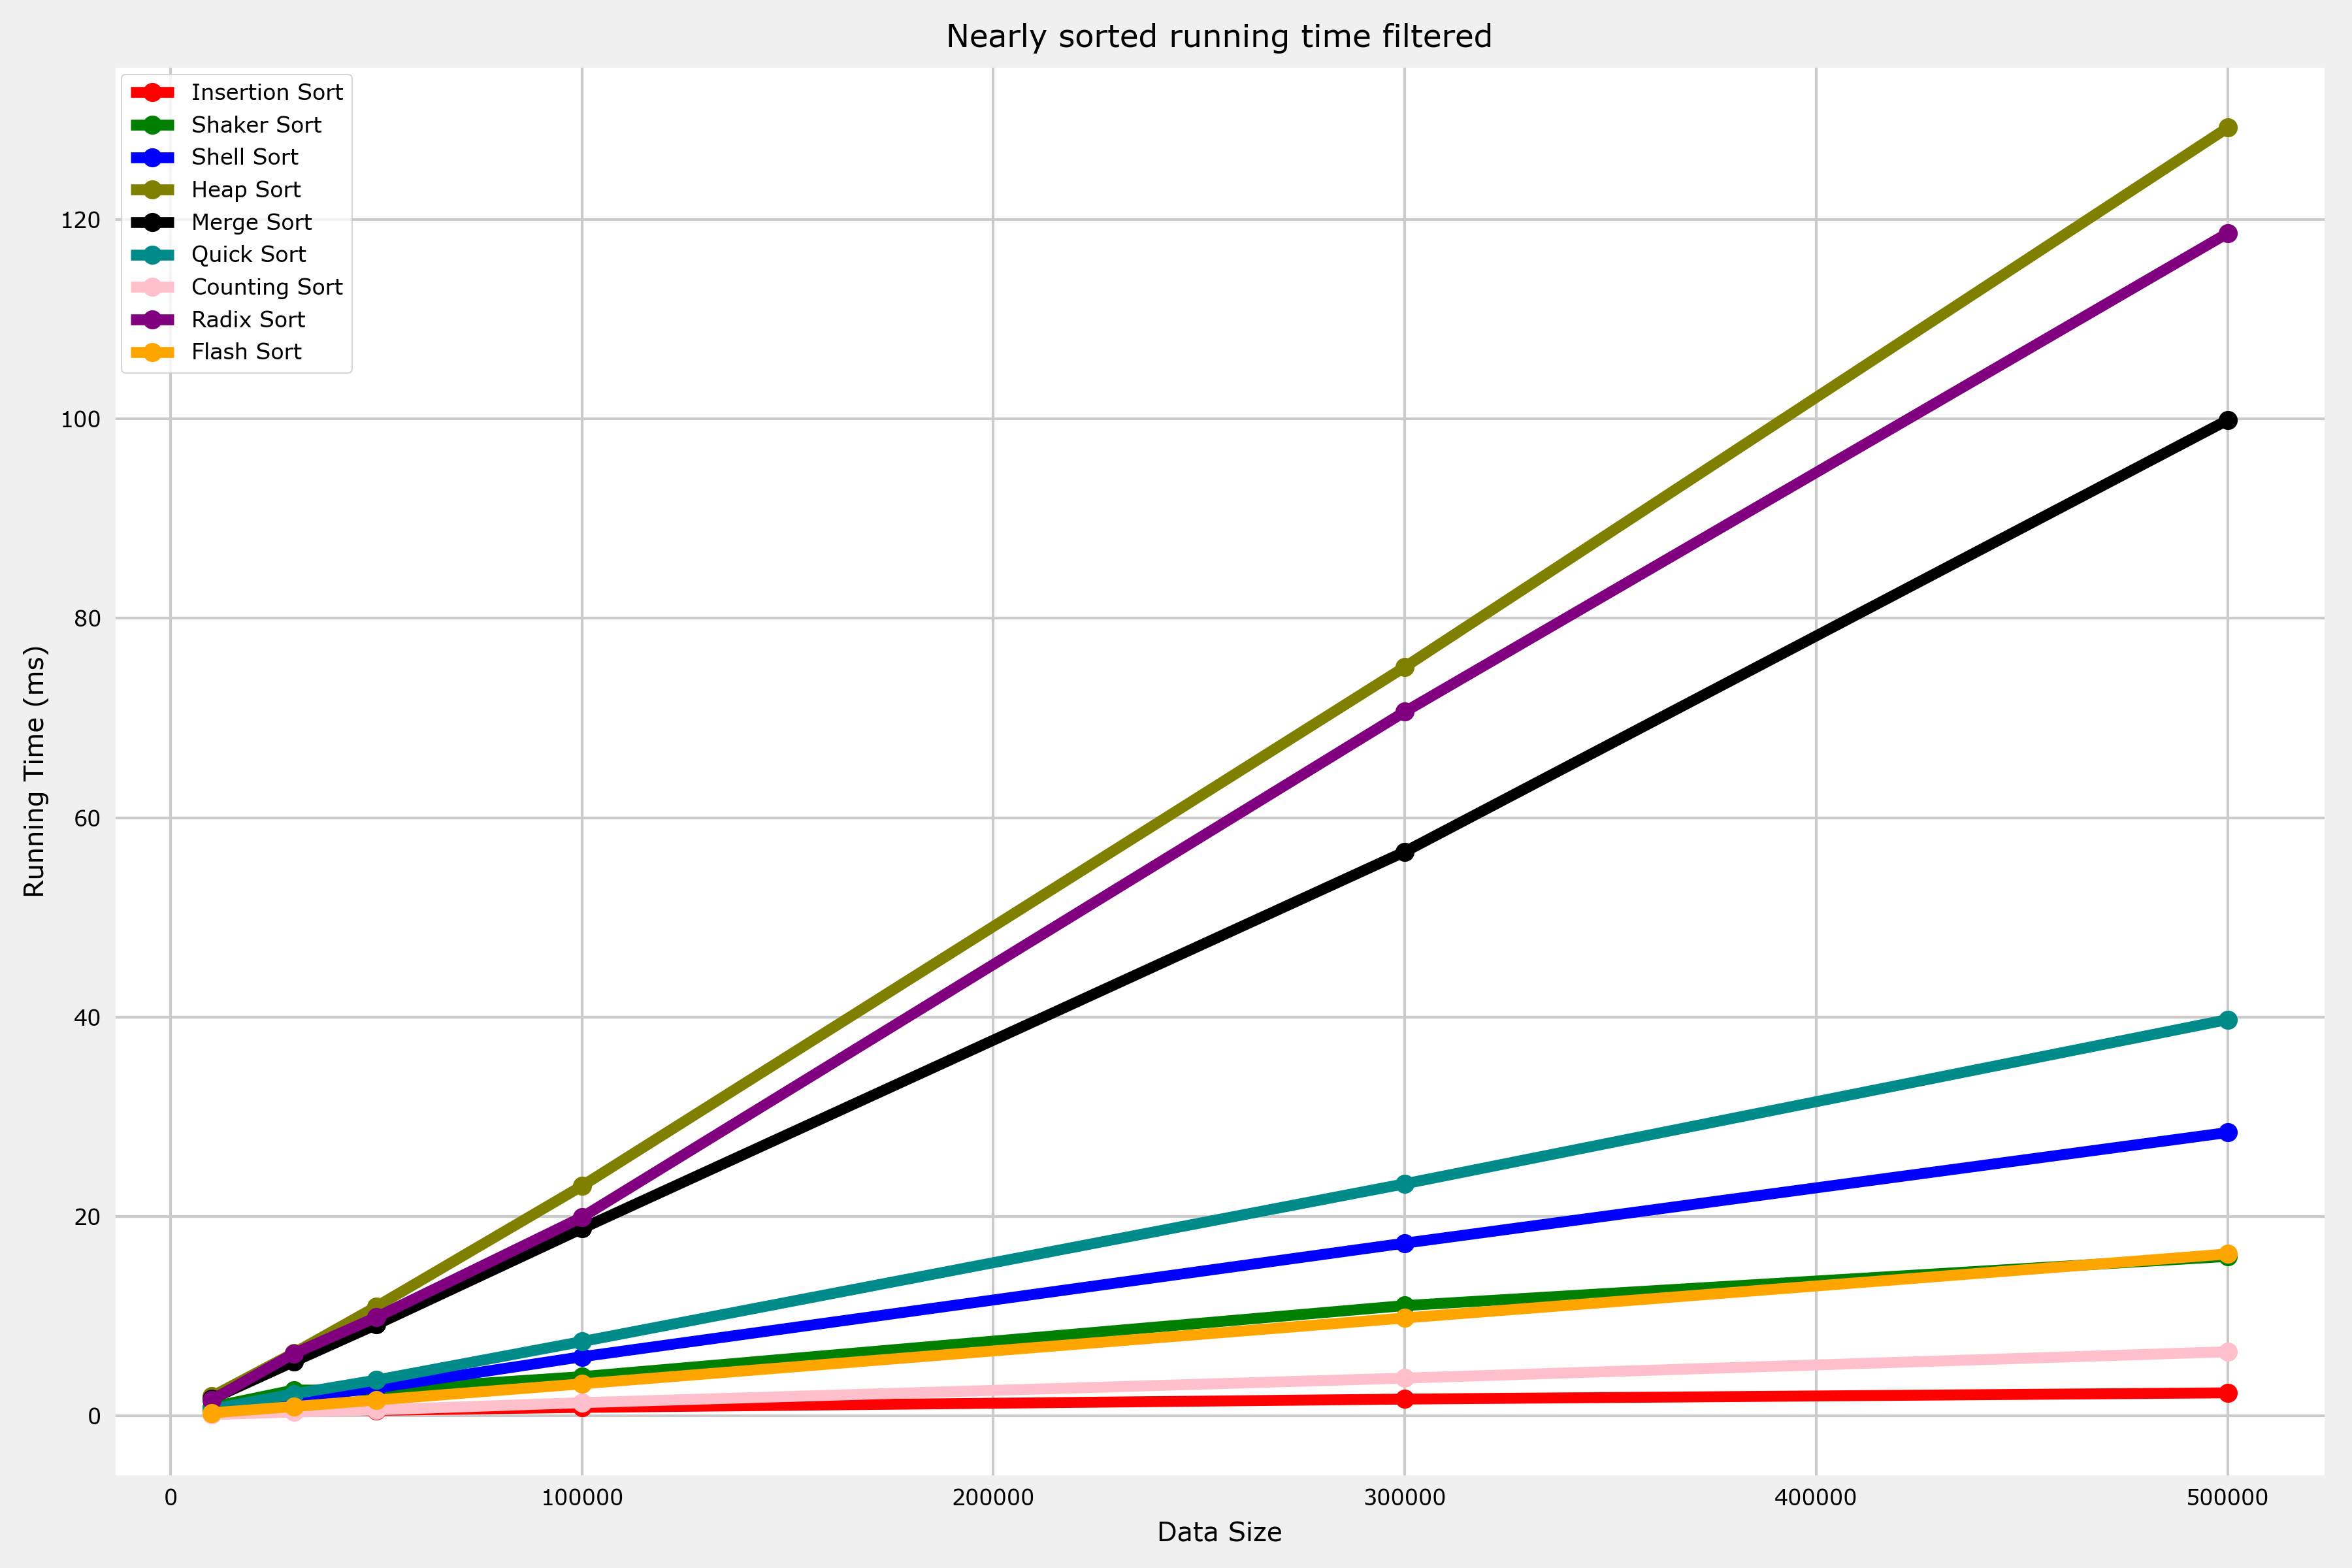
\includegraphics[width=0.8\textwidth]{exprimental_result/images/nearly_sorted_running_time_filtered.png}
    \caption{Thời gian chạy của 11 thuật toán với dữ liệu gần sắp xếp hoàn chỉnh sau khi loại bỏ outlier}
\end{figure}


\paragraph{3. Dữ liệu được sắp xếp}
\begin{figure}[H]
    \centering
    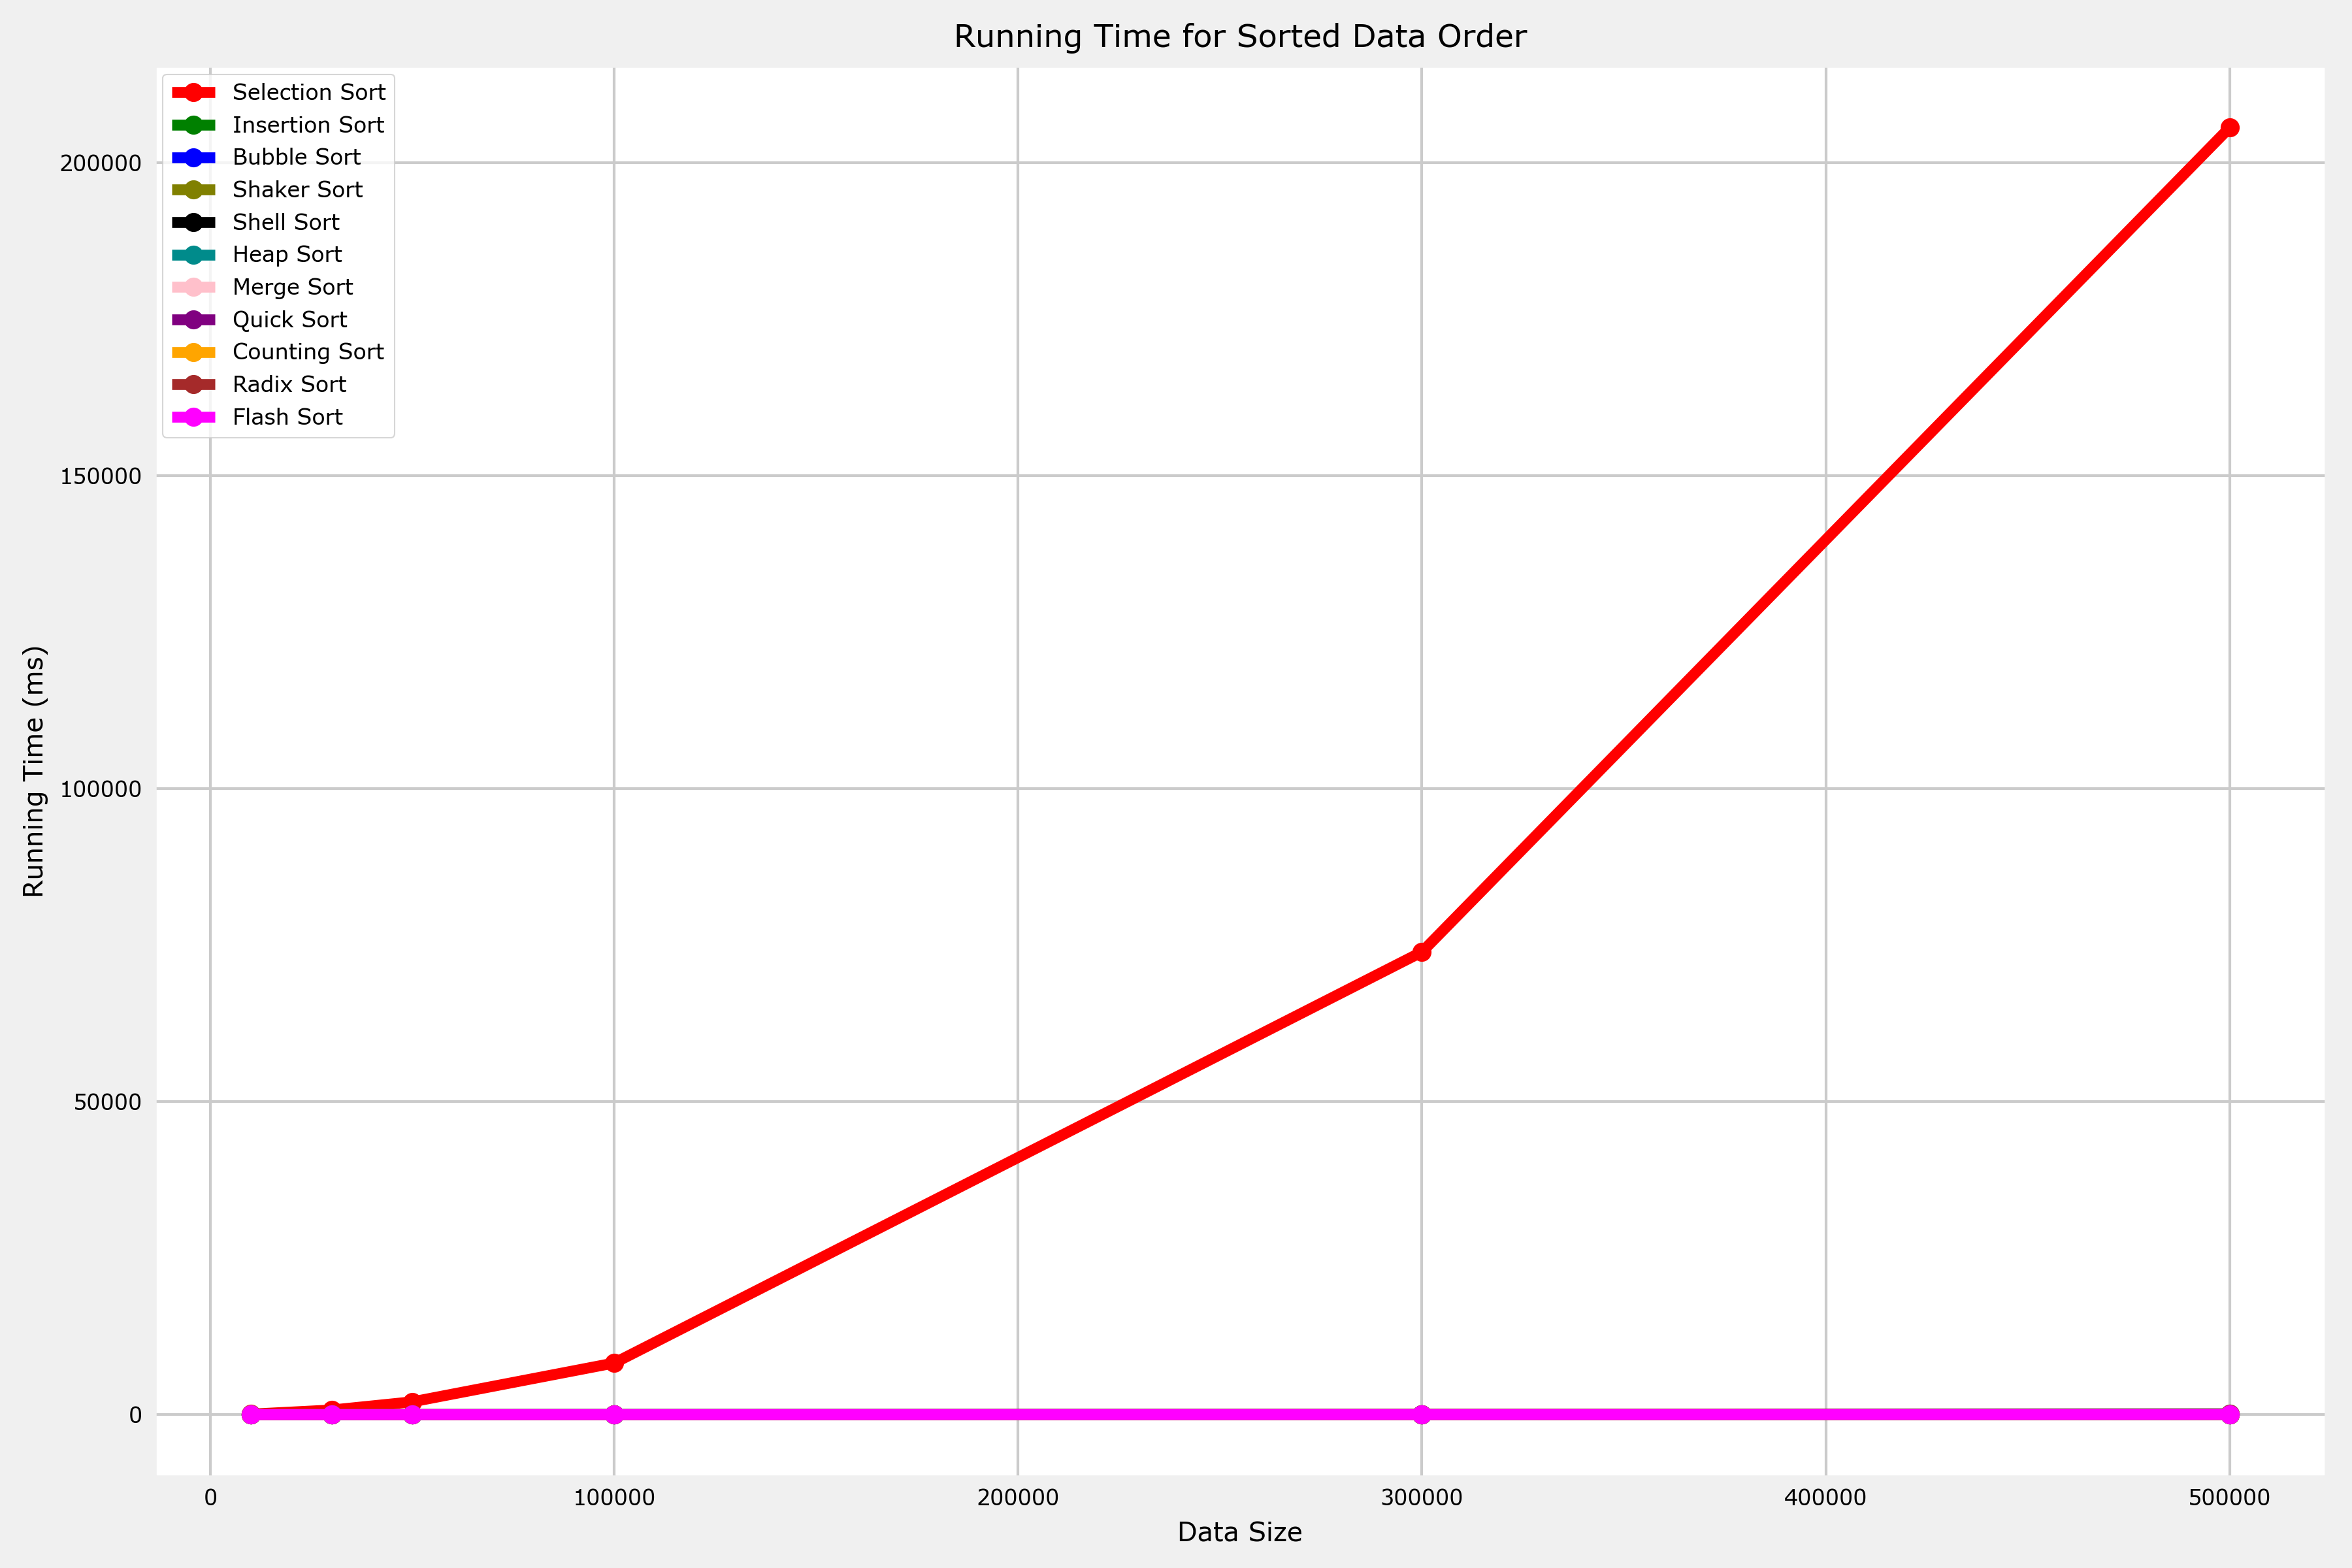
\includegraphics[width=0.8\textwidth]{exprimental_result/images/sorted_running_time.png}
    \caption{Thời gian chạy của 11 thuật toán với dữ liệu được sắp xếp}
\end{figure}

\begin{figure}[H]
    \centering
    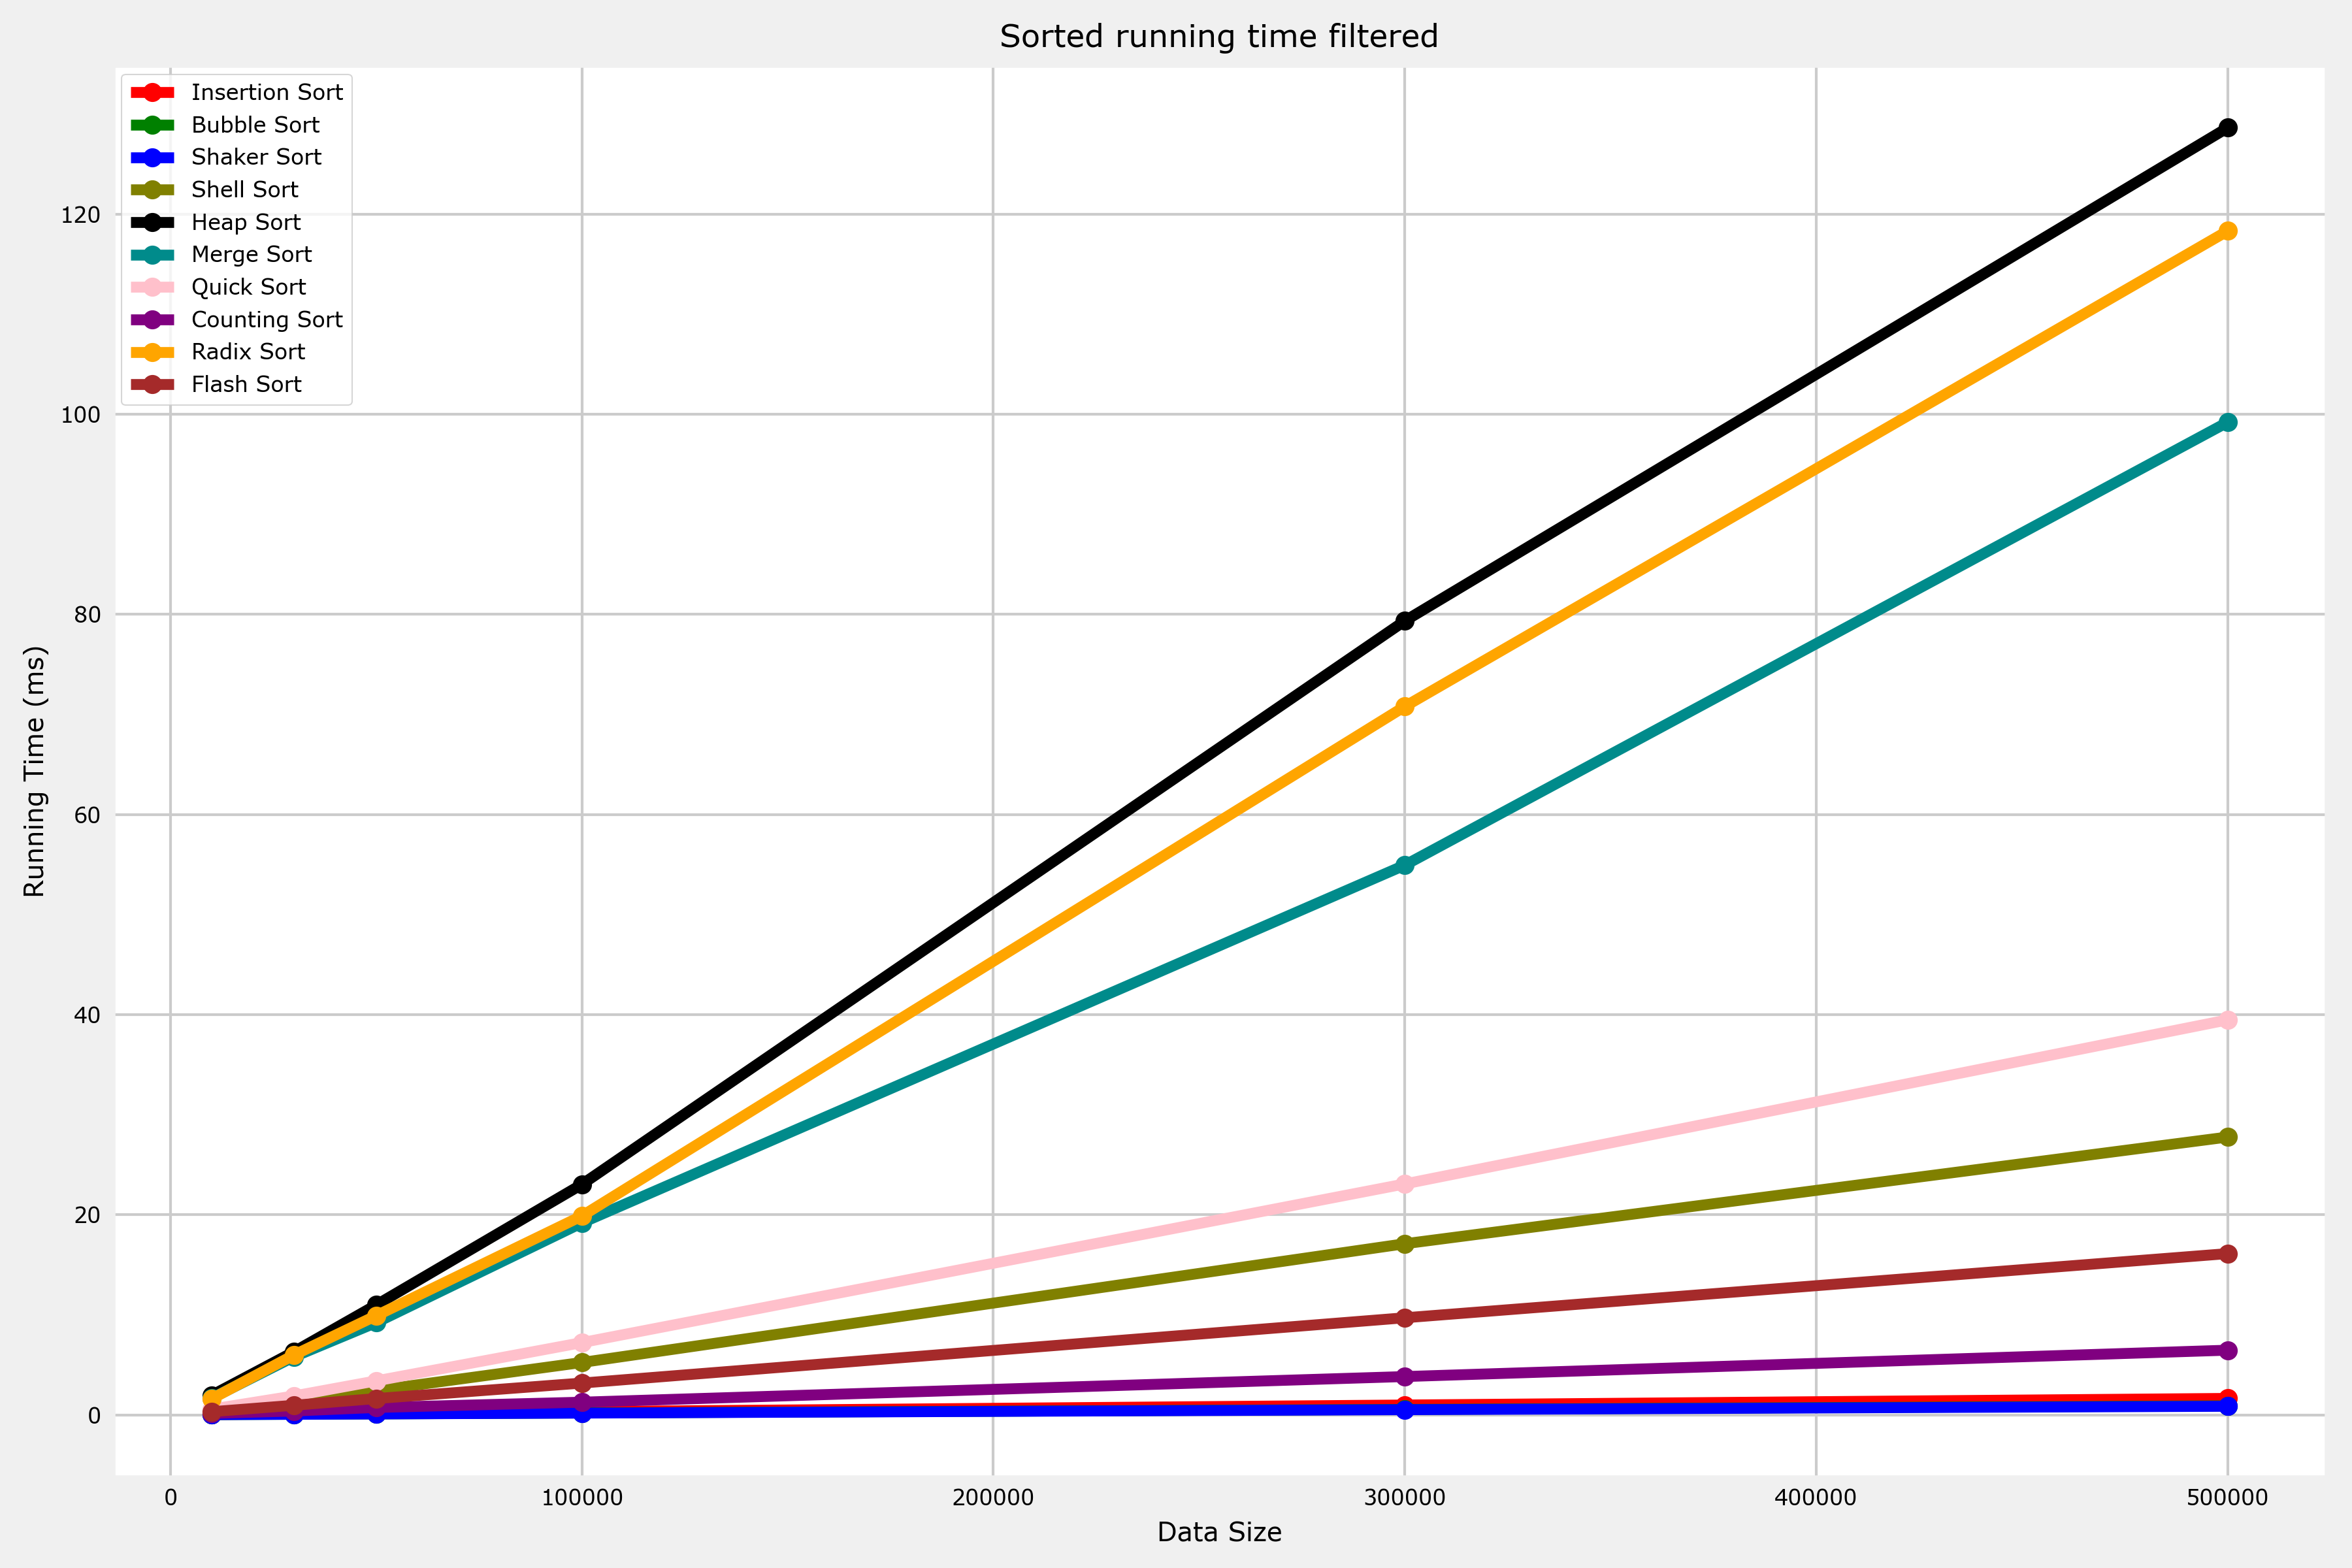
\includegraphics[width=0.8\textwidth]{exprimental_result/images/sorted_running_time_filtered.png}
    \caption{Thời gian chạy của 11 thuật toán với dữ liệu được sắp xếp sau khi loại bỏ outlier}
\end{figure}




\paragraph{4. Dữ liệu đảo ngược}
\begin{figure}[H]
    \centering
    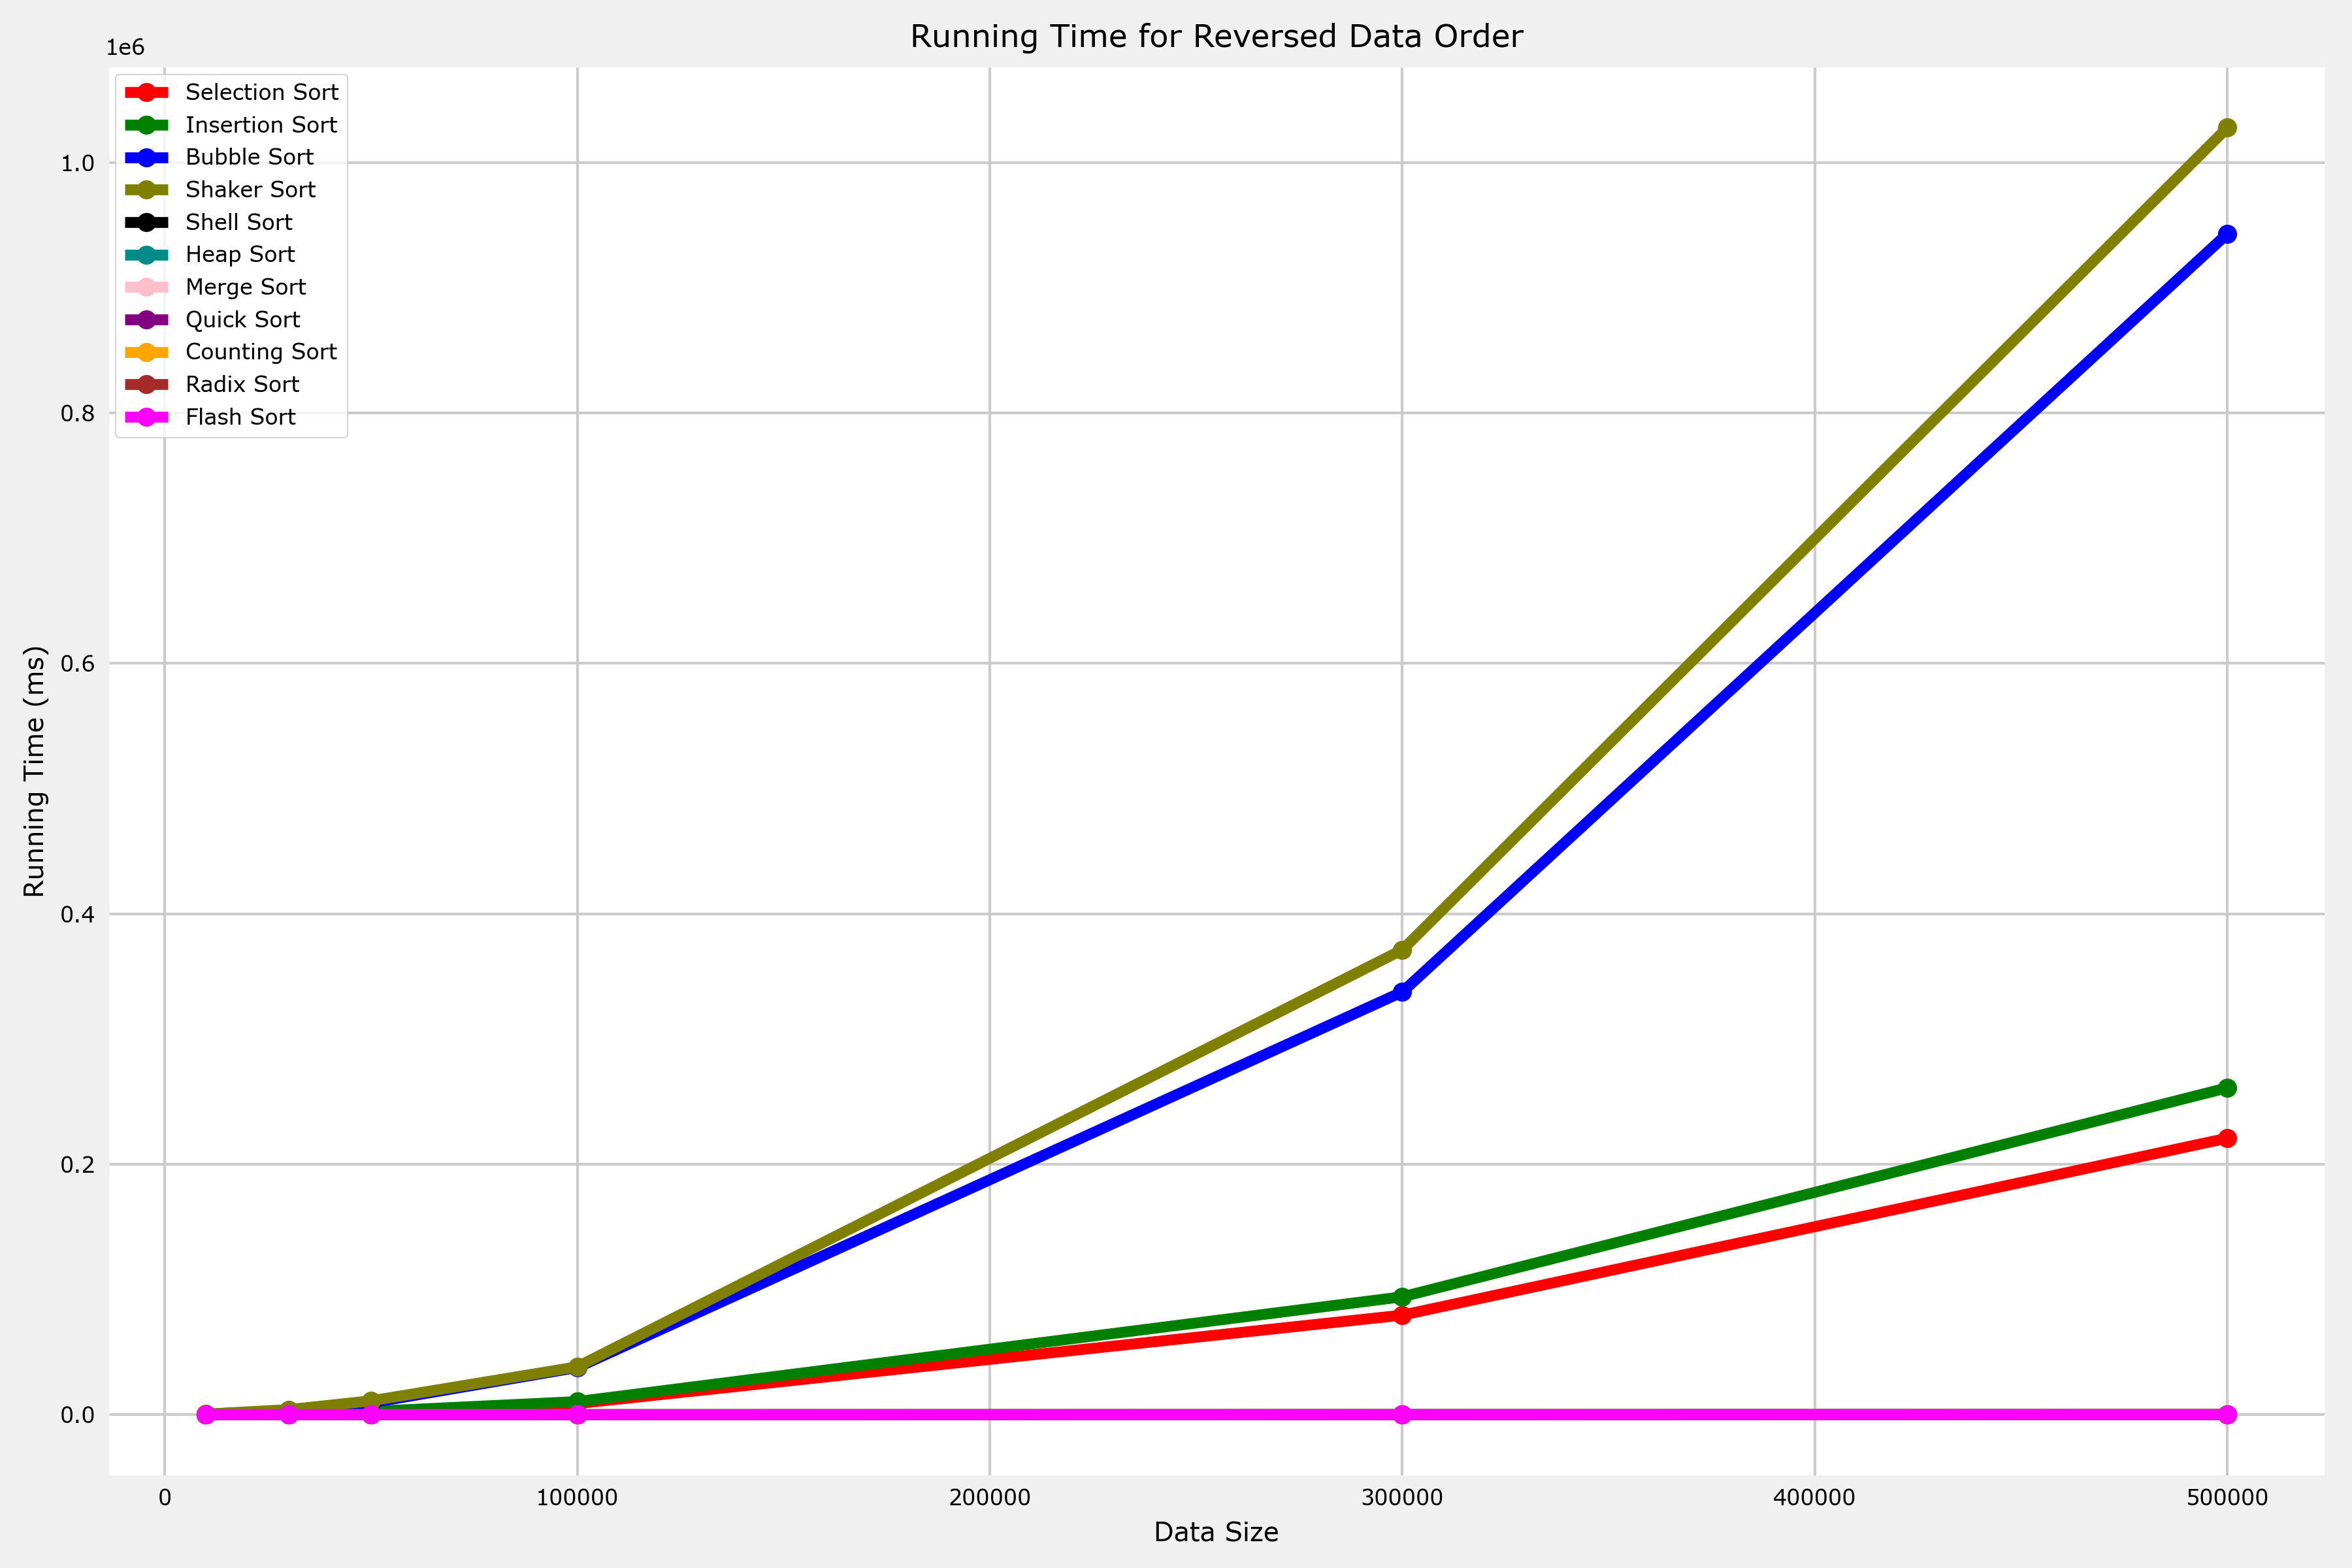
\includegraphics[width=0.8\textwidth]{exprimental_result/images/reversed_running_time.png}
    \caption{Thời gian chạy của 11 thuật toán với dữ liệu đảo ngược}
\end{figure}

\begin{figure}[H]
    \centering
    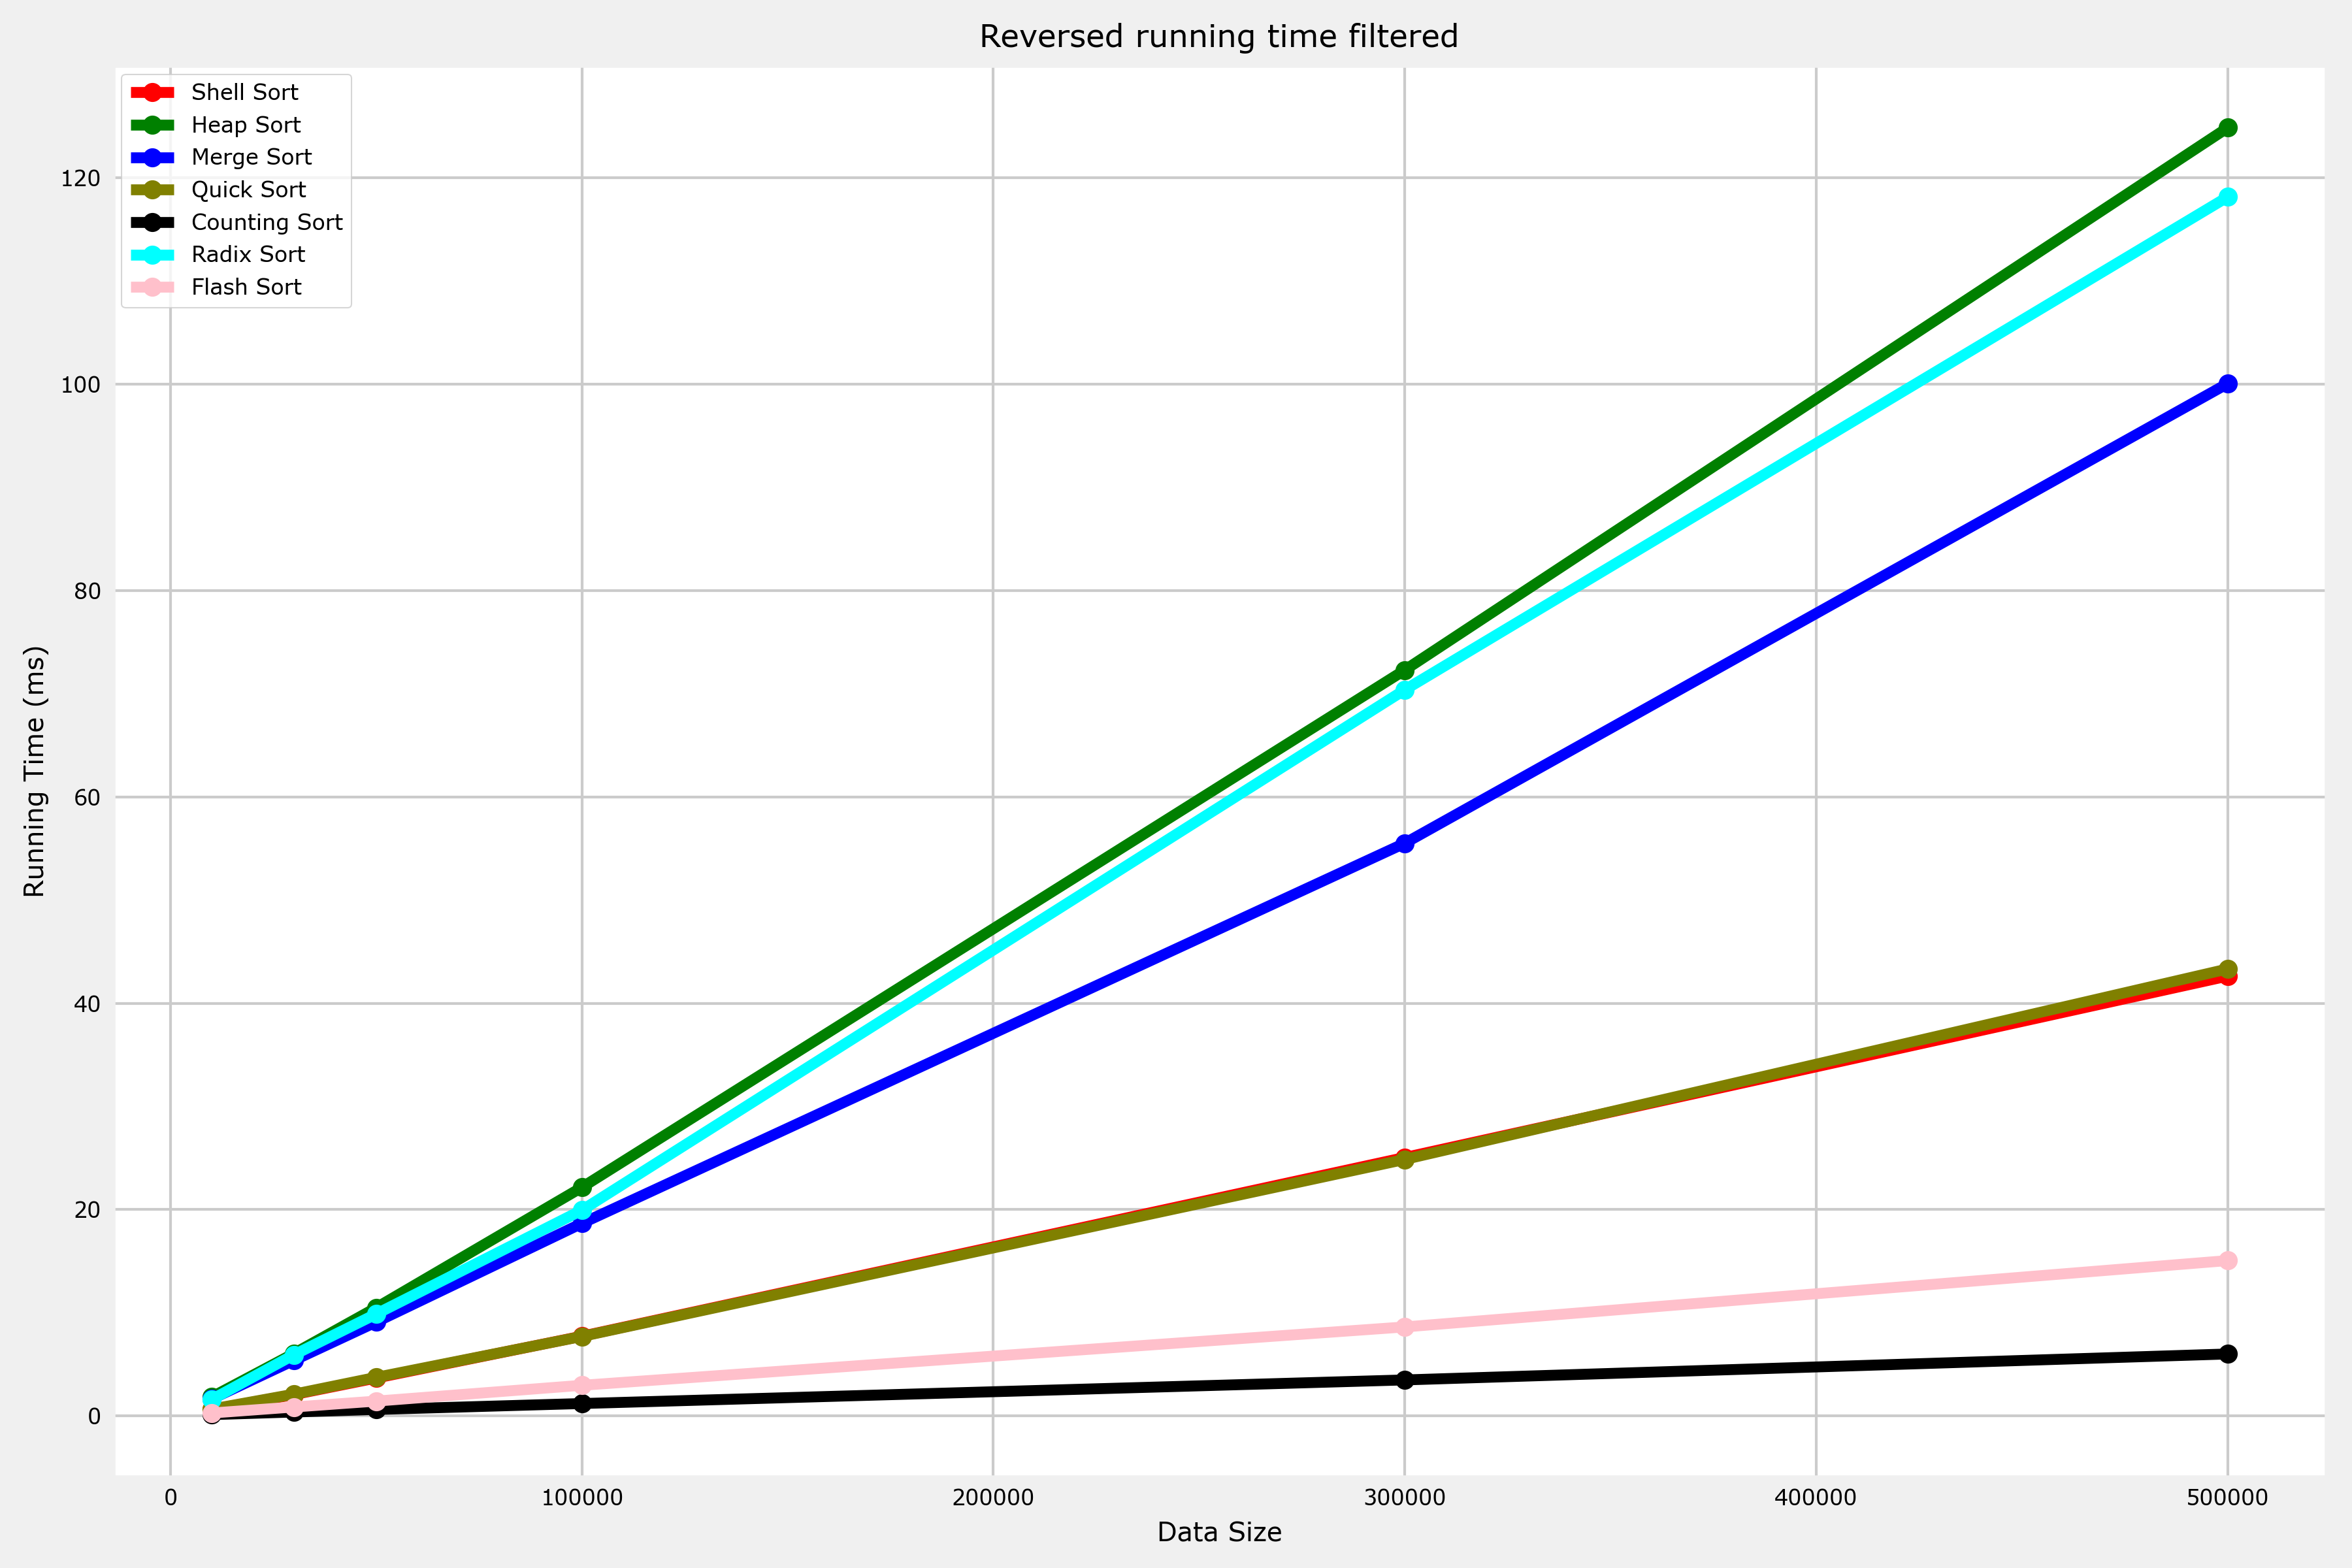
\includegraphics[width=0.8\textwidth]{exprimental_result/images/reversed_running_time_filtered.png}
    \caption{
        Thời gian chạy của 11 thuật toán với dữ liệu đảo ngược sau khi loại bỏ outlier
    }
\end{figure}










